\documentclass[aspectratio=169,t]{beamer}
\usepackage[czech]{babel}
\usepackage[utf8]{inputenc}
\usepackage[T1]{fontenc}
\usepackage{booktabs}
\usepackage{diagrams}
\usepackage{amsmath}
\bibliographystyle{unsrt}
\usetheme[workplace=fi]{MU}
\title{Vektorové reprezentace ve vyhledávání znalostí}
\subtitle{Vector Space Representations in Information Retrieval}
\author[V.\ Novotný]{Vít Novotný \\ witiko@mail.muni.cz}
\institute[FI MU]{Faculty of Informatics, Masaryk University}
\date{\today}
\subject{Presentation Subject}
\keywords{the, presentation, keywords}
\date{6.\ února 2017}

% Macro definitions.
\let\abbr\relax
\let\term\emph
\begin{document}

\begin{frame}[plain]
\maketitle
\end{frame}

\begin{frame}{Obsah}
\setbeamertemplate{section in toc}[sections numbered]
\tableofcontents
\end{frame}

\section{Úvod}
\begin{frame}[label=introduction]{Úvod}
\begin{itemize}
  \item<1-> V~rámci výzkumné skupiny Math Information Retrieval (\abbr{MIR})
    jsem se ve spolupráci s~firmou RaRe Technologies zúčastnil třetího kola
    projektu \alert<1>{\abbr{TA} \abbr{ČR} Omega}.
  \item<2-> Cíl byl vyvinout \alert<2-3>{segmentující vyhledávač}
    nestrukturovaných textových dokumentů\only<2-3>:\only<4->.
  \only<4->{%
  \item<4-> V rámci projektu jsem dostal možnost prezentovat náš výzkum na \abbr{ACL}~2017.
  \item<5-> V návaznosti na výzkum prezentovaný na \abbr{ACL}~2017 jsem
    provedl \alert<5->{sérii experimentů}, které jsou předmětem této diplomové
    práce:
  \begin{enumerate}
    \item<6-> U~vyhledávačů, které musí vždy navrátit celé dokumenty a nikoliv
      pouze segmenty, lze \alert<6>{agregací nalezených segmentů} zlepšit
      kvalitu výsledků oproti hledání bez segmentace.
    \item<7-> Rozšířením standardního vektorového modelu o neortogonalitu mezi
      bázovými vektory lze \alert<7>{modelovat synonymitu slov} a docílit
      dalšího zlepšení kvality výsledků.
  \end{enumerate}}
\end{itemize}
\only<1>{\vspace*{6cm}}
\only<2>{\STqueryingdiagram[f]}
\only<3>{\hspace*{-10.5cm}\STqueryingdiagram[f]\vspace*{0.5cm}}
\only<4->{\vspace*{2cm}}
\end{frame}

\section{Datová sada}
\begin{frame}<1-4>[label=dataset]{Datová sada}
\begin{itemize}
\item<1-> V rámci obou experimentů jsem využil datovou sadu pro úlohu 3
  (zodpovídání dotazů) z~ročníků 2016 a 2017 soutěže SemEval.
\item<2-> Datové sady pro podúlohu 3a obsahují \alert<2-6>{vlákna s dotazem a
  prvními deseti komentáři} spolu s~anotací, jestli \alert<2-6>{je komentář
  relevantní k~dotazu}.
  \begin{itemize}
    \item<3-> Mike Godwin roku 1991 formuloval empirické pravidlo, že
      „s~rostoucí délkou UseNetové diskuze se pravděpodobnost přirovnání
      zmiňujícího nacisty nebo Hitlera blíží k~jedné.“
    \item<4-> Na základě tohoto pravidla jsem formuloval a vyvrátil hypotézu, že
      \alert<4>{pravděpodobnost výskytu relevantních komentářů na jednotlivých
      pozicích je rovnoměrná}.
  \end{itemize}
\item<5-> Datové sady pro podúlohu 3b obsahují dotazy a \alert<5-6>{pro každý
  dotaz deset vláken} spolu s anotací, jestli se \alert<5-6>{vlákno týká dotazu}.
  Vlákna řadíme podle podobnosti k~dotazu.
  \begin{itemize}
    \item<6-> Tyto datové sady byly použity pro evaluaci v obou následujících
      experimentech.
  \end{itemize}
\end{itemize}
\end{frame}

\begin{frame}[c]
\begin{figure}
\vfill
\begin{center}
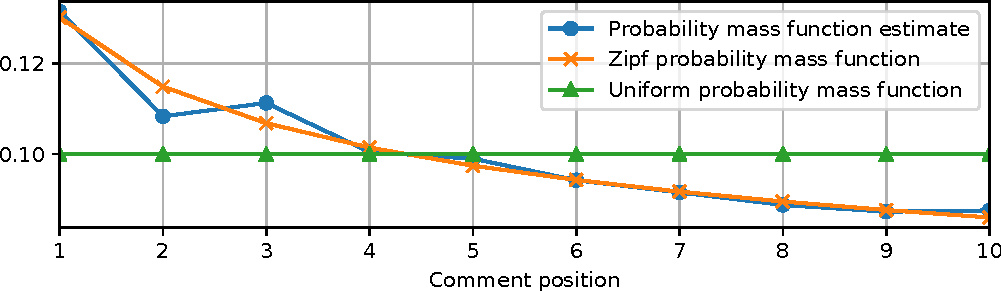
\includegraphics[scale=0.8]{figs/quality-evaluation-1}
\end{center}
\caption{Odhad pravděpodobnostní funkce $P(\text{na pozici }i\mid\text{relevantní})$
  vyobrazený modře spolu s~pravděpodobnostními funkcemi Zipfova (oranžový graf)
  a rovnoměrného rozdělení (zelený graf).}
\end{figure}
\end{frame}

\againframe<4->{dataset}

\section{Segmentované vyhledávání}
\begin{frame}<1-5>[label=segmentation]{Segmentované vyhledávání}
\begin{itemize}
  \item<1-> Vyhledávač navržený v projektu Omega indexuje a navrací
    \alert<1>{tématicky koherentní segmenty dokumentů}. Vyhledávače však často
    musí navracet celé dokumenty.
  \item<2-> V rámci experimentu jsem vyhledávač rozšířil o komponentu, která
    \alert<2>{agreguje podobnost segmentů vůči dotazu} do odhadu podobnosti
      dokumentu vůči dotazu\only<2>:\only<3->.
    \begin{itemize}
      \only<-2>{\item[]}
      \only<3->{%
      \item<3-> \alert<3>{Vlákna představují dokumenty}, \alert<3>{dotaz a
        komentáře uvnitř vláken představují segmenty}.
      \item<4-> S ohledem na analýzu datových sad podúlohy 3a je hlavním agregačním
        mechanismem \alert<4-5>{vážený průměr s~vahou $i^{-1}$ pro komentář na
        pozici $i$}. Tento mechanismus \alert<4>{porazil vítěze} ročníků 2016 a
        2017 soutěže SemEval.
      \item<5-> Pro srovnání byl otestován i \alert<5>{vyhledávač bez segmentace},
        který analogickým způsobem \alert<5>{váží jednotlivá slova dokumentu}.
        Tento vyhledávač \alert<5>{byl poražen baseline výsledkem}.
      \item<6-> Pro srovnání byl otestován i \alert<6>{vyhledávač bez segmentace},
        který \alert<6>{z~vlákna zachovává pouze úvodní dotaz}. Tento
        vyhledávač \alert<6>{porazil baseline výsledek}, \alert<6>{ale ne
        vítěze soutěže}.}
    \end{itemize}
\end{itemize}
\only<1>{\vspace*{5cm}}
\only<2>{\vspace*{-0.8cm}\hspace*{-14cm}\STqueryingdiagram[t]}
\only<3->{\vspace*{0.5cm}}
\end{frame}

\begin{frame}[c]
\begin{figure}
\vfill
\begin{center}
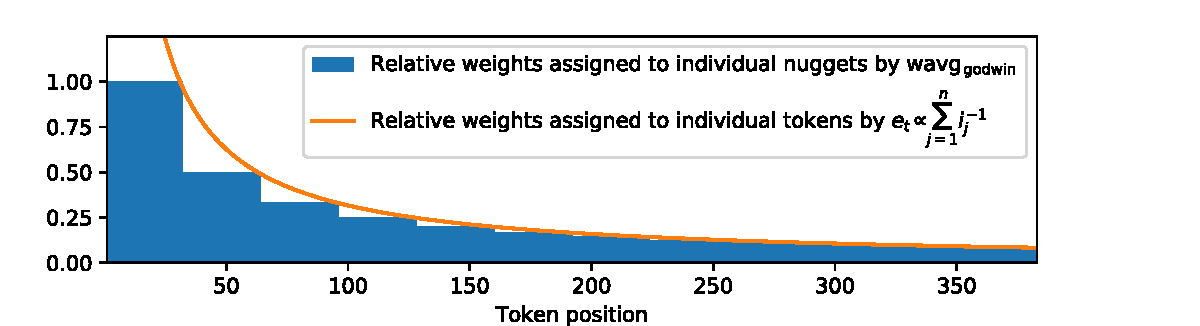
\includegraphics[trim={0.8cm 0.0cm 2.8cm 0.5cm}, scale=0.8]{figs/quality-evaluation-4}
\end{center}
\caption{Poměrný dopad jednotlivých slov v dokumentu na výsledný odhad
  podobnosti při váženém průměru jednotlivých segmentů (modře vyplněný graf) a
  při váženém průměru jednotlivých slov (oranžový graf).}
\end{figure}
\end{frame}

\againframe<5->{segmentation}

\section{Modelování synonymie}
\begin{frame}<1-3>[label=similarity]{Modelování synonymie}
\begin{itemize}
  \item<1-> Vyhledávač navržený v projektu Omega reprezentuje dokumenty pomocí
    \alert<1>{slovních histogramů (bag of words)}, nebo pomocí \alert<1>{histogramů
    témat (\abbr{LSA})}.
  \item<2-> \alert<2>{Podobnost} dvou dokumentů \alert<2>{je dána kosinem úhlu}
    mezi histogramy.
  \item<3-> S ohledem na modelování synonymie slov trpí obě reprezentace neduhy:
    \begin{itemize}
      \item<3-> Standardní model předpokládá, že \alert<3>{histogramy zadávají
        souřadnice v~ortogonální bázi}.
      \item<4-> LSA \alert<4>{shlukuje slova} do témat výhradně \alert<4>{na
        základě jejich souvýskytu} v~segmentech.
    \end{itemize}
  \item<5-> Vyhledávač jsem rozšířil, aby \alert<5>{nepředpokládal, že
    bázové vektory jsou ortogonální}.
    \begin{itemize}
      \item<6-> \alert<6>{Skalární součin} bázových vektorů je \alert<6>{zadán
        Gramovou maticí $\mathbf S$} velikosti $n$.
      \item<7-> Popsal jsem, kdy lze \alert<7>{vypočítat kosinus úhlu
        v~konstatním čase}.
      \item<8-> Popsal jsem, jak \alert<8>{v~čase $\mathcal O(n^3)$ vypočítat matici
        přechodu do ortogonální báze}.
      \item<9-> Zadefinoval jsem trojici matic $\mathbf S$, které
        \alert<9>{modelují různé rysy synonymie}.
      \item<10-> Diskutoval jsem \alert<10>{implementaci ve vektorových databázích
        a~invertovaných indexech}.
      \item<11-> Dosáhl jsem \alert<11>{srovnatelných výsledků s~vítězi} ročníků 2016 a
        2017 soutěže SemEval.
    \end{itemize}
\end{itemize}
\end{frame}

\begin{frame}[c]
\begin{figure}
\vfill
\begin{center}
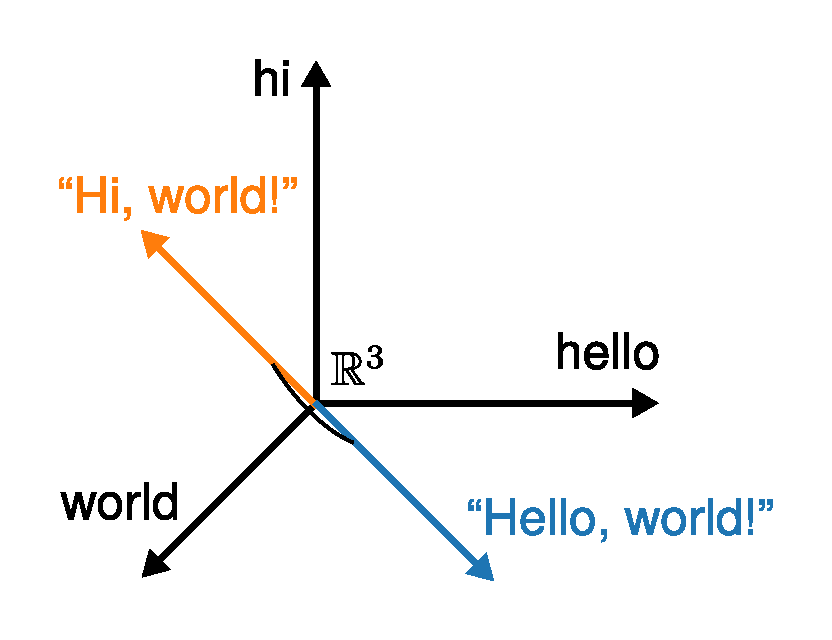
\includegraphics[scale=0.6]{figs/cosine}
\end{center}
\caption{Standardní model předpokládá, že histogramy zadávají souřadnice
  v~ortogonální bázi.}
\end{figure}
\end{frame}

\againframe<3-5>{similarity}

\begin{frame}[c]
\begin{figure}
\vfill
\begin{center}
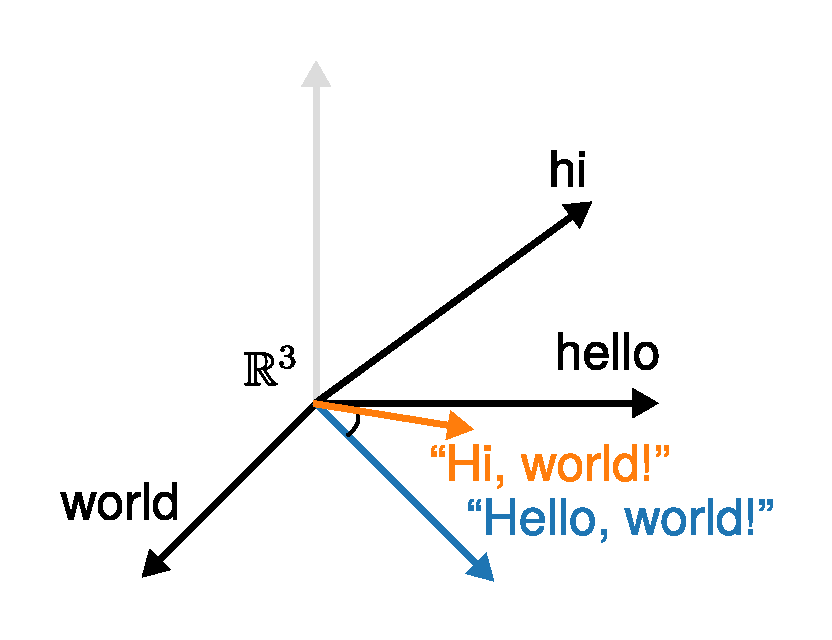
\includegraphics[scale=0.6]{figs/soft-cosine}
\end{center}
\caption{Rozšířený model předpokládá, že histogramy zadávají souřadnice
  v~libovolné bázi.}
\end{figure}
\end{frame}

\againframe<5->{similarity}

\section{Závěr a budoucí výzkum}
\begin{frame}[label=introduction]{Závěr a budoucí výzkum}
\begin{itemize}
  \item<1-> Objevil jsem \alert<1-2>{statisticky významný vztah mezi pozicí
    příspěvku} v~diskuzi \alert<1-2>{a jeho relevancí} k~tématu diskuze na
    datových sadách soutěže SemEval.
  \begin{itemize}
    \item<2-> Budoucí výzkum by měl toto pozorování potvrdit na
      \alert<2>{nezávislých datových sadách}.
  \end{itemize}
  \item<3-> Popsal jsem \alert<3-4>{dvojici technik}, pomocí kterých lze
    \alert<3-4>{zlepšit kvalitu výsledků} běžného vyhledávače \alert<3-4>{na
    úroveň \term{state-of-the-art}} výsledků ze soutěže SemEval.
  \begin{itemize}
    \item<4-> Budoucí výzkum by se měl zaměřit na evaluaci systému, který
      \alert<4>{implementuje obě techniky současně}, ideálně na nezávislých
      datových sadách.
  \end{itemize}
  \item<5-> Kapitolu o agregaci jsem nezávisle zaslal na konferenci \abbr{ECIR}~2018.
  \begin{itemize}
    \item<6-> Jeden z recenzentů \alert<6>{navrhl článek na \term{best paper award}}.
    \item<7-> Článek byl \alert<7>{zamítnut} kvůli údajné \alert<6-7>{nedostatečné
      obecnosti použitých datových sad}.
  \end{itemize}
  \item<8-> Načrtnul jsem, jak by mohl agregační mechanismus \alert<8>{využívat
    strojové učení}.
  \item<9-> Neortogonální model jsem \alert<9>{zanesl do knihovny Gensim pro
    modelování jazyka}.
\end{itemize}
\end{frame}

\begin{frame}[label=thanks, plain]
\vfill
\centerline{Děkuji vám za pozornost.}
\vfill
\end{frame}

\begin{frame}<-2>[label=rebuttal-opponent]{Reakce na posudek oponenta}
\begin{quote}
K~obhajobě práce mám na autora jednu otázku: V~kapitole 4.6 je popsána \alert<1>{metoda
expanze dotazů}, která umožňuje nalézt i takové dokumenty, které neobsahují
žádné termy z~původního dotazu. Nabízí se však také \alert<1>{alternativní přístup},
\alert<1>{který by expandoval texty dokumentu} a indexoval je potom i pod
expandovanými termy. \alert<1>{Jsou oba přístupy ekvivalentní}, nebo je některý
z~nich pro information retrieval výhodnější?
\end{quote}
\only<2->{%
\begin{itemize}
  \item<2-> V sekci 4.6 popisuji, jak lze \alert<2-4>{neortogonální model
    implementovat pomocí expanze dotazu} na straně klienta.
  \begin{itemize}
    \item<3-> Na serveru lze použít \alert<3>{běžný invertovaný index},
      který uchovává původní dokumenty.
    \item<4-> Na klientovi lze použít \alert<4>{rozličné matice $\mathbf S$}
      bez změny obsahu indexu.
  \end{itemize}
  \item<5-> Při expanzi indexovaných dokumentů \alert<5>{lze stále použít běžný
    invertovaný index}, ale \alert<5>{dochází až k $n$-násobnému nárůstu objemu
    uchovávaných dat} a \alert<5>{změna matic $\mathbf S$ vyžaduje opětovnou
    indexaci} všech dokumentů.
\end{itemize}}
\end{frame}

\begin{frame}[c]
\begin{figure}
\vfill
\begin{align*}
  d_2 = \text{``}&\text{I did enact Julius Caesar: I was killed i' the Capitol''}, \\
  d_3 = \text{``}&\text{\footnotesize Give\textvisiblespace{}unto\textvisiblespace{}Caesar Brutus\textvisiblespace{}Cassius choreographers\textvisiblespace{}Bosco Julius\textvisiblespace{}Caeser}\index{.d3@$d_3$|emph} \\
  &\text{\footnotesize therefore\textvisiblespace{}unto\textvisiblespace{}Caesar Marcus\textvisiblespace{}Antonius Caesarion
    Gallic\textvisiblespace{}Wars} \\
  &\text{\footnotesize Marcus\textvisiblespace{}Crassus Antoninus Catiline Seleucus
    Gaius\textvisiblespace{}Julius\textvisiblespace{}Caesar} \\
  &\text{\footnotesize Theodoric Marcus\textvisiblespace{}Tullius\textvisiblespace{}Cicero unto\textvisiblespace{}Caesar
    emperor\textvisiblespace{}Nero} \\
  \vdots \phantom{{}=} & \\
  &\text{\footnotesize Benjamin Kenneth Philip Marcus Arthur Carl Fred Edward Jonathan Eric} \\
  &\text{\footnotesize Frank Anthony William Richard Robert enact Capitol killed Ididn't} \\
  &\text{\begingroup\footnotesize honestly myself I I my we the
    'd 'm did was\endgroup''}.
\end{align*}
\caption{Expanze dotazu na straně klienta.}
\end{figure}
\end{frame}

\againframe<2->{rebuttal-opponent}
\againframe{thanks}

\end{document}
